\documentclass[12pt]{article}

\usepackage[numbers,sort&compress]{natbib}
\usepackage{graphicx}
\usepackage{authblk}

\usepackage[utf8]{inputenc}
\usepackage[T1]{fontenc}
\usepackage[french]{babel}
%\usepackage{french} 


\usepackage{macros}
\usepackage{aas_macros}


%% \usepackage[utf8]{inputenc}
%% \usepackage[T1]{fontenc}
%% \usepackage[french]{babel}
%% %\usepackage{french}

%% \usepackage{times}
\usepackage{geometry}
\geometry{a4paper, portrait, margin=2cm}

\usepackage{enumitem,amssymb}
\setenumerate{itemsep=0mm}
\usepackage{ragged2e}
%% \usepackage{graphicx}
%% \usepackage{comment}
\usepackage{multicol}
%\usepackage[usenames]{xcolor} %used for font color              
\definecolor{xlinkcolor}{cmyk}{1,1,0,0}
\usepackage{url}
\usepackage[
 colorlinks=true,    % false: boxed links; true: colored links 
 linkcolor=xlinkcolor,     % color of internal links            
 citecolor=xlinkcolor,     % color of links to bibliography
 filecolor=xlinkcolor,  % color of file links 
 urlcolor=xlinkcolor,      % color of external link
 final=true
]{hyperref}
%% \usepackage[super,sort&compress]{natbib}
%% \usepackage{enumitem}
%% \setenumerate{itemsep=0mm}

\newcommand{\Comment}[3]{\textcolor{#1}{(#2: #3)}} 
\newcommand{\ADW}[1]{\Comment{blue}{ADW}{#1}} % Alex Drlica-Wagner 
\newcommand{\KB}[1]{\Comment{orange}{KB}{#1}} % Keith Bechtol

%% \newlist{thematic}{itemize}{8}
%% \setlist[thematic]{label=$\square$}
%% \usepackage{pifont}
\newcommand{\cmark}{\ding{51}}%
\newcommand{\xmark}{\ding{55}}%
\newcommand{\done}{\rlap{$\square$}{\raisebox{2pt}{\large\hspace{1pt}\cmark}}%
\hspace{-2.5pt}}
\newcommand{\wontfix}{\rlap{$\square$}{\large\hspace{1pt}\xmark}}

\setlength{\parskip}{0.5em}

\begin{document}

\begin{raggedright} 
% part of template, but does not look good
  \large
  Contribution aux prospectives IN2P3 2020\hfill ~ \linebreak
\end{raggedright}
\normalsize

\centering{\Large \bf Identification de la Matière Noire à l'ère du grand relevé optique LSST}

%\vspace{1cm}
%% \noindent \textbf{Thematic Areas:} \hspace*{58pt} $\square$ Planetary Systems \hspace*{12pt} $\square$ Star and Planet Formation  \hfill ~\linebreak
%% $\blacksquare$ Formation and Evolution of Compact Objects \hspace*{31pt} $\blacksquare$ Cosmology and Fundamental Physics \hfill ~ \linebreak
%%   $\square$  Stars and Stellar Evolution \hspace*{1pt} $\square$ Resolved Stellar Populations and their Environments \hspace*{40pt} \hfill ~\linebreak
%%   $\square$    Galaxy Evolution   \hspace*{45pt} $\square$             Multi-Messenger Astronomy and Astrophysics \hspace*{65pt} \hfill ~ \linebreak

% Author list file generated with: mkauthlist.py UNKNOWN 
% python code/mkauthlist.py -f -s -j emulateapj -a data/order.csv data/astro2020_endorsers_trimmed_merged.csv tmp.tex 

\def\altaffilmark#1{\textsuperscript{#1}}
\def\affil#1{\noindent #1 \\}

%% \noindent \textbf{Principal Authors:} 
%% Keith Bechtol\altaffilmark{1}, \href{mailto:kbechtol@wisc.edu}{kbechtol@wisc.edu} (UW Madison)\\
%% Alex~Drlica-Wagner\altaffilmark{2,3,4}, \href{mailto:kadrlica@fnal.gov}{kadrlica@fnal.gov} (Fermila/KICP/UChicago)
%
%\noindent Name:	
% \linebreak						
%Institution:  
% \linebreak
%Email: 
% \linebreak
%Phone:  

\begin{flushleft}
  {\bf Auteur principal}  Johann Cohen-Tanugi\\
  {\bf Institution}  LUPM, université de Montpellier et CNRS/IN2P3, Montpellier, France\\
  {\bf email} johann.cohen-tanugi@umontpellier.fr
\end{flushleft}       


\noindent {\bf Co-auteurs :}
\begin{raggedright}
\small
Julien Lavalle\altaffilmark{1}, Marc Moniez\altaffilmark{3}, Eric Nuss\altaffilmark{1}
%\setlength{\parskip}{\baselineskip}
\end{raggedright}

\noindent {\bf Endosseurs :}
\begin{raggedright}
\small
Dominique Boutigny\altaffilmark{5},
Céline Combet\altaffilmark{2},
David Maurin\altaffilmark{2},
Emmanuel Moulin\altaffilmark{4},
Vivian Poulin\altaffilmark{1},
Cécile Renault\altaffilmark{2}
%\setlength{\parskip}{\baselineskip}
\end{raggedright}

%\begin{multicols}{2}
\scriptsize
%\parskip=4pt

\affil{$^{1}$ LUPM, université de Montpellier et CNRS/IN2P3, Montpellier, France}
\affil{$^{2}$ LPSC, université de Grenoble et CNRS/IN2P3, Grenoble, France}
\affil{$^{3}$ LAL, université Paris-Orsay et CNRS/IN2P3, Orsay, France}
\affil{$^{4}$ SPP, CEA Centre de Saclay, Gif-sur-Yvette, France}
\affil{$^{5}$ LAPP, université Savoie Mont Blanc, Annecy-le-vieux, France}
\normalsize
%\end{multicols}
%\parskip=8pt


%\noindent \textbf{Abstract:}
\abstract{Les observations astrophysiques fournissent aujourd'hui encore la seule mesure empirique robuste de la matière noire.
  Dans la prochaine décennie, ces observations continueront de sonder de manière unique des régions de l'espace des paramètres, tout en guidant d'autres efforts expérimentaux.
  Cette contribution résume les nombreuses observations que LSST ({Large Synoptique Survey Telescope}) rendra possibles et qui pourront contraindre la nature de la matière noire.
  Elle dessine succinctement la richesse des résultats qui peuvent être obtenus, en étroite collaboration avec ces autres efforts expérimentaux, et souligne la pertinence de ce programme de recherche au sein de l'IN2P3.\footnote{Cette contribution s'inspire largement du {\it  science white paper for Astro 2020} \citep{2019BAAS...51c.207B}, lui-même un résumé du livre blanc de la communauté \citep{drlica-wagner_2019_lsst_dark_matter}, auxquels plusieurs des auteurs principaux de cette contribution ont participé.}\footnote{Des informations supplémentaires sur le groupe de travail ``Matière noire et LSST'' sont disponibles à l'adresse suivante : \href{https://lsstdarkmatter.github.io/}{https://lsstdarkmatter.github.io/}.}
  \\
\vspace{0.5cm}
  \noindent Cette contribution fait l'objet d'une soumission au GT04 et au GT06.
}

%\pagebreak

% Insert your white paper text here (max 5 pages inc. figs).

%\vspace{-1em}
\subsection*{Introduction}

Près d'un siècle après la découverte de sa présence dans le cosmos, la matière noire demeure une énigme parmi les plus importantes de la physique fondamentale. Depuis plusieurs décennies, un très large programme expérimental sur plusieurs continents, auquel l'IN2P3 participe fortement, a cherché à déterminer la nature de cette matière noire. \`A ce jour, les seules observations probantes demeurent néanmoins les observations astrophysiques, qui révèlent les effets gravitationnels de sa présence. Toute révolution future dans notre compréhension de la nature de la matière noire s'appuiera à n'en pas douter sur les observations, outils, et expertises des trois communautés de la physique des particules, de la cosmologie, et de l'astronomie.

Dans ce contexte, le {\it Large Synoptic Survey Telescope} (LSST) fournira au milieu de la prochaine décennie une plateforme remarquable pour étudier la physique du secteur sombre. Initialement conçu comme un {\it ``Dark Matter Telescope''} \citep{Tyson:2001}, LSST fournira de nombreuses observations pour tester de manière précise certains aspects du modèle \LCDM et pour élucider la connection entre galaxies lumineuses et `toile' cosmique ({\it cosmic web}) de la matière noire. Non seulement il n'est plus aujourd'hui possible d'isoler cette \emph{distribution macroscopique} de la \emph{description microscopique} de la matière noire, mais de surcroît certaines caractéristiques microscopiques ne sont accessibles que par des observations astrophysiques. 
Ainsi, l'étude de la matière noire, de l'énergie noire, des neutrinos massifs, de l'univers primordial etc..., nécessite pour la décennie à venir une approche complémentaire aussi bien du point de vue expérimental que du point de vue théorique. L'IN2P3, de par sa couverture thématique et technique, est idéalement placé pour participer efficacement à un programme global sur le sujet, en s'appuyant sur LSST pour tester un large éventail de modèles théoriques viables, tels que matière noire interagissant avec elle-même, matière noire froide ou `tiède', matière noire avec interactions baryoniques, matière noire ultra-légère, modèles axioniques généralisés, et trous noirs primordiaux. LSST donnera accès à des observations de satellites locaux et de traînées stellaires de la Voie Lactée, de systèmes à lentillage fort, d'amas de galaxies isolés ou en interaction, de micro-lentillage, de populations stellaires et de la structure à grande échelle de l'Univers. L'IN2P3 est également engagé sur des projets qui fournissent les moyens ou bien de produire des particules de matière noire, ou bien de détecter directement ou indirectement leurs interactions, et peut donc assurer un rôle moteur pour maintenir la synergie adéquate entre ces axes expérimentaux fortement complémentaires. Il est utile de rappeler ici que cette vision globale où LSST jouera un rôle crucial a été identifiée dans plusieurs livres blancs et rapports outre-atlantique \citep{Astro2010,1310.8642, 1310.5662, 1305.1605,P5Report,1604.07626,1802.07216,Battaglieri:2017aum}. Après un bref rappel de la `zoologie' actuelle des modèles de matière noire, nous faisons ci-dessous un tour d'horizon des sondes accessibles à LSST, puis nous concluons sur la pertinence d'un programme de l'IN2P3 sur l'identification de la matière noire qui s'appuie sur la contribution de l'institut à LSST.

\vspace{-1em} \subsection*{Modèles de Matière Noire} \vspace{-0.5em}

Si la décennie passée a cherché avant tout à détecter les signatures attendues d'un candidat de type WIMP ({\it weakly interactive massive particle}), la décennie qui s'ouvre devant nous fait face, du fait de l'échec de ces tentatives, à une pléthore de modèles phénoménologiques proposant une réponse à la question de la nature de la matière noire. S'il est essentiel de concevoir l'instrumentation dédiée à la détection du plus grand nombre possible de ces candidats, il est important de rappeler que les observations astrophysiques sondent la physique de la matière noire au travers de son impact sur la formation des structures tout au long de l'histoire de l'Univers. Aux larges échelles, les données d'observations sont très bien décrites par l'ajustement statistique d'un modèle cosmologique qui inclut une composante non relativiste, non collisionnelle, et froide (CDM pour {\it cold dark matter}). Toutefois, de nombreuses extensions au modèle standard fournissent des candidats matière noire viables, qui dévieraient du scénario CDM standard, en particulier aux plus petites échelles. En effet les propriétés fondamentales d'une particule de matière noire -masse, sections efficaces d'interactions, couplage aux particules du modèle standard, évolution temporelle- peuvent laisser une trace détectable sur la distribution macroscopique de matière noire. Soutenu par la poursuite des efforts théoriques et l'appui de suivis observationnels sur d'autres télescopes, LSST sera sensible à plusieurs classes distinctes de modèles. Nous mentionnons ici quelques exemples.

\noindent \textbf{Matière Noire de type particule} LSST, combiné avec d'autres observations, pourra apporter des indices importants pour caractériser la section efficace d'auto-interaction et/ou de diffusion avec des baryons, la masse, le taux d'annihilation ou de désintégration, etc... De telles mesures viendront compléter et guider les efforts de détection directe, indirecte, et sur collisionneur.

\noindent \textbf{Matière Noire de type ondes} Les ALP ({\it Axion-Like Particles}) et autres candidats dits ``ultra-légers'' sont une alternative crédible aux candidats plus conventionnels. LSST sera en mesure d'apporter des contraintes distinctes sur la masse minimale de tels candidats, ainsi que sur le couplage ALP-particules du modèle standard.

\noindent \textbf{Objets compacts} Cette classe de candidats est fondamentalement différente des deux premières. En particulier les trous noirs primordiaux (PBH pour {\it Primordial Black Hole}) ne sont accessibles à l'étude que par des observations astrophysiques, et des contraintes portées sur leur abondance fourniraient directement des contraintes sur l'amplitude des fluctuations de densité initiales, en plus de fournir des indices uniques sur la physique à ultra-haute énergie.

%Fundamental properties of dark matter---e.g., particle mass, self-interaction cross section, coupling to the Standard Model, and time evolution---can imprint themselves on the macroscopic distribution of dark matter in a detectable manner. With supporting theoretical efforts and follow-up observations, LSST will be sensitive to several distinct classes of dark matter models, including particle dark matter, field dark matter, and compact objects (\tabref{models}).

\vspace{-1em} \subsection*{Sondes de Matière Noire} \vspace{-0.5em}
LSST pourra s'appuyer sur un grand nombre de sondes pour caractériser la nature de la matière noire. Une table interactive est disponible en ligne\footnote{à l'adresse \href{https://lsstdarkmatter.github.io/dark-matter-graph/}{https://lsstdarkmatter.github.io/dark-matter-graph/}}, et nous n'évoquons ci-dessous que les grandes classes de sondes.\\
\noindent {\bf Masse minimale des galaxies, et caractérisation des halos}
Si on en croit le modèle cosmologique standard, le spectre de masse des halos devrait être invariant d'échelle jusqu'à des masses planétaires, voire en deça \citep[par exemple]{Green:2003un,2005Natur.433..389D,1412.5930}. Ces petites échelles peuvent être supprimées dans le cadre de modèles alternatifs au paradigme CDM.
Les observations actuelles contraignent de manière satisfaisante le spectre de masse des halos jusqu'à $10^{10}\Msun$ environ, et les galaxies les plus petites connues permettent d'inférer l'existence de halos de masse $\roughly 10^8 \Msun - 10^9 \Msun$ \citep{2017MNRAS.467.2019R,behroozi2018,Jethwa:2018,Kim:2017iwr,Nadler:2018,1807.07093}. 
LSST va étendre le décompte du nombre de galaxies satellites très peu brillantes en orbite autour de la Voie Lactée, et va même permettre de chercher des systèmes très peu lumineux dans tout le volume local. Ces observations à la limite du seuil de formation stellaire permettront de contraindre l'abondance des halos de masse $\sim10^8 \Msun$.

Par ailleurs, LSST pourra descendre plus bas encore dans l'échelle des masses, en deça du seuil de formation stellaire, grâce aux traînées stellaires et aux lentilles fortes. Dans le premier cas, des sous-structures galactiques de masse $10^5$--$10^6 \Msun$ seront détectables par leur perturbation de la structure des traînées stellaires \citep[][]{erkal2016,bovy:2017}, et il est attendu que LSST découvre de nouvelles traînées, améliore le contraste de densité de celles qui sont connues, et surtout fournisse des cas individuels plus éloignés du coeur de la Galaxie. Dans le deuxième cas, LSST découvrira de nombreux nouveaux systèmes fortement lentillés, permettant d'atteinde un échantillon de plusieurs milliers de quasars lentillés \citep{O+M10} et plusieurs dizaines de milliers de galaxies lentillées \citep{Collett2015}, permettant d'accéder à l'abondance et à la distribution de masse des sous-halos des galaxies massives et des halos isolés le long de la ligne de visée.

\noindent {\bf Profils de Halo}
Les interactions non gravitationnelles de la matière noire avec elle-même, que prédisent certains modèles de physique des particules au-delà du modèle standard, pourraient produire des coeurs de halo dont la densité ne dépend pas du rayon \citep[coeurs `plats', ][]{Spergel:1999mh} et/ou des profils strictement sphériques \citep{Peter:2013}.
Dans ce contexte, le lentillage faible galaxie-galaxie devrait permettre à LSST de distinguer les coeurs plats pour des galaxies naines à faible décalage vers le rouge et de masse $M_\text{halo} = 3\times10^9\,h^{-1}\Msun$. Par ailleurs, l'étude des profils de densité des amas massifs de galaxies, ainsi que des systèmes de deux amas en coalescence, renseignera sur les sections efficaces de diffusion de l'ordre de $\sigmam \sim 0.1-1 \cmg$ pour des candidats matière noire interagissant avec eux-mêmes. Enfin, l'étude des profils de halo en fonction de leur masse permettra de contraindre des mécanismes de diffusion qui dépendent de la vitesse. 

\noindent {\bf Objets Compacts}
Le caractère synoptique du relevé de LSST offre la possibilité d’observer des passages d'objets compacts devant d’autres étoiles, soit par occultation, soit par effet de microlentille gravitationnelle,
sur des échelles de temps courtes ($\roughly 30 \second$) et longues ($\roughly1-10 \unit{ans}$)\citep{1509.04899}. 
Avec une cadence optimale, LSST pourrait également étendre les contraintes sur la fraction de PBH jusqu'à $\roughly0.03\%$ du budget matière noire, pour des masses $\gtrsim 10^{-1} \Msun$. Des observations astrométriques seront extrêmement utiles pour lever la dégénerescence des paramètres et mesurer la masse de trous noirs individuels, si ils existent, et donc fournir une fenêtre d'observation sur l'Univers primordial.

\noindent {\bf Anomalie de perte d'énergie}
L'astrophysique stellaire modélise l'évolution des étoiles, et en particulier les mécanismes de transfert radiatif, de manière détaillée. L'observation des populations stellaires permet alors de confronter ces modèles et de déceler éventuellement des anomalies dans les pertes radiatives, qui signaleraient la présence d'un mécanisme non conventionnel de perte d'énergie, en particulier dû à la présence de matière noire. Par exemple des particules de faible masse couplées aux champs du modèle standard fournissent naturellement un canal supplémentaire de pertes radiatives. En particulier, des mesures de la fonction de luminosité des naines blanches, des géantes rouges, ou des supernovae gravitationnelles peuvent contraindre le couplage axion-électron.

\noindent {\bf Structure à grande échelle} LSST produira la carte la plus large et la plus détaillée de l'évolution de la distribution de masse durant les derniers dix milliards d'années. Cette structuration à grande échelle dépend de la quantité totale de matière noire, de la fraction de reliques `chaudes' qui la composent, et des couplages éventuels entre la matière noire et l'énergie noire. Sur ce dernier point, la taille et la profondeur du relevé de LSST pourrait permettre d'étudier les corrélations spatiales du secteur sombre en déterminant les paramètres de l'énergie noire indépendamment dans différentes régions du ciel \citep{0902.2590}.

%% \begin{figure}[t]
%% \centering
%% 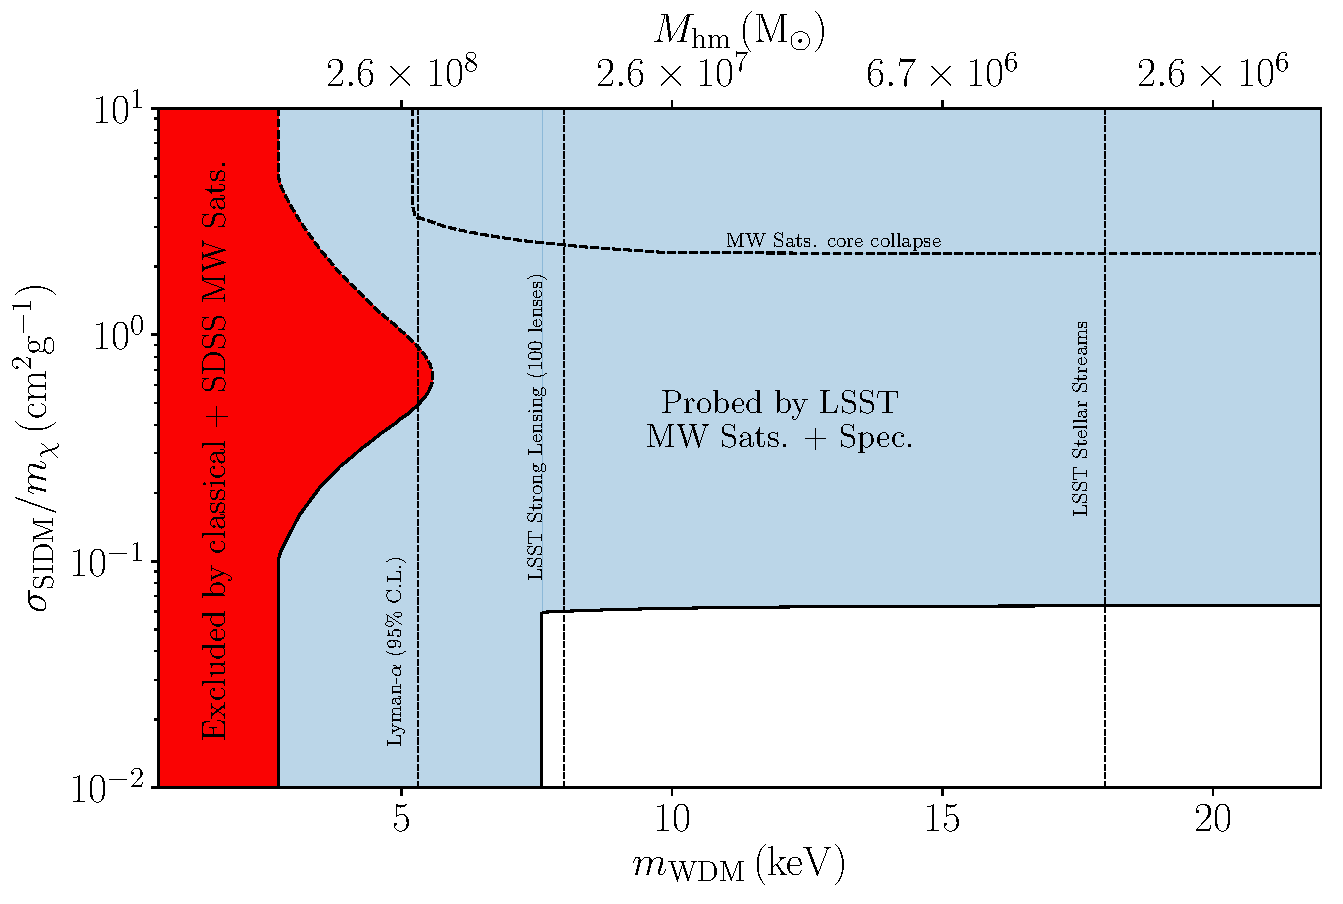
\includegraphics[width=0.53\columnwidth]{figures/SIDM_WDM_figw_coll.pdf}
%% 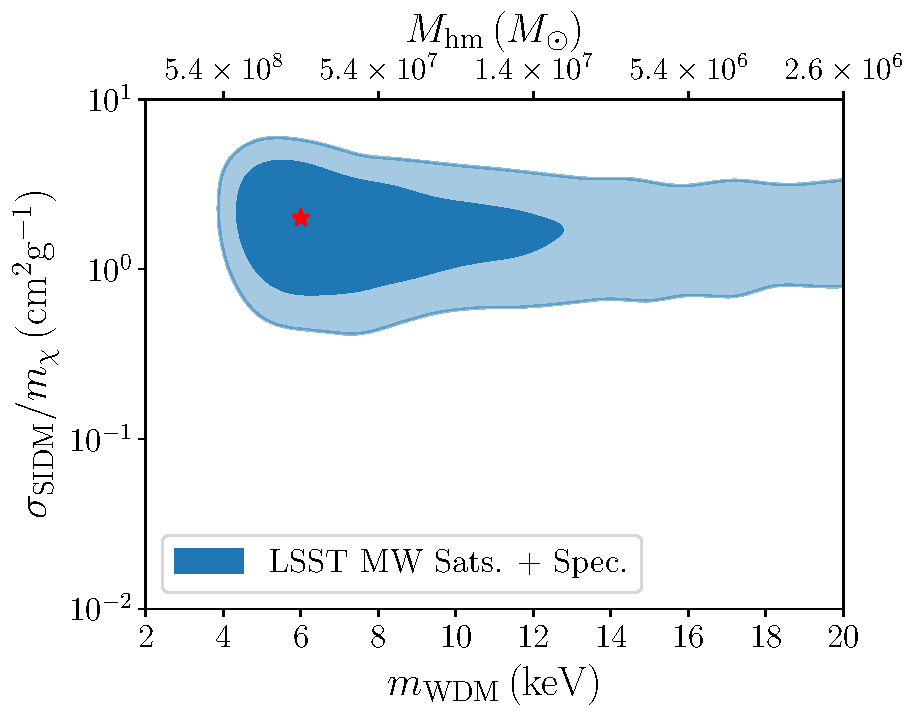
\includegraphics[width=0.46\columnwidth]{figures/WDM_SIDM_discovery_test.pdf}
%% \caption{\emph{Left}: Projected joint sensitivity to WDM particle mass and SIDM cross section from LSST observations of dark matter substructure. 
%% \emph{Right}: Example of a measurement of particle properties for a dark matter model with a self-interaction cross section and matter power spectrum cut-off just beyond current constraints ($\sigmam = 2 \cmg$ and $\mWDM = 6\keV$, indicated by the red star) \citep{drlica-wagner_2019_lsst_dark_matter}. Complementary observations can break degeneracies among dark matter models that have the same approximate behavior on small scales but differ in detail.}
%% \end{figure}


%% \begin{table}[ht]
%% \footnotesize
%% \begin{center}
%% \begin{tabular}{l c c c}
%% \hline 
%% Model & Probe & Parameter & Value \\
%% \hline 
%% \hline
%% Warm Dark Matter  & Halo Mass & Particle Mass & $m \sim 18 \keV$ \\
%% Self-Interacting Dark Matter & Halo Profile & Cross Section & $\sigmam \sim 0.1\text{--}10\cm^2/\g$ \\
%% Baryon-Scattering Dark Matter & Halo Mass & Cross Section & $\sigma \sim 10^{-30} \cm^2$ \\
%% Axion-Like Particles & Energy Loss & Coupling Strength & $g_{\phi e} \sim 10^{-13} $ \\
%% Fuzzy Dark Matter & Halo Mass & Particle Mass & $m \sim 10^{-20} \eV$  \\
%% Primordial Black Holes  & Compact Objects & Object Mass & $M > 10^{-4} \Msun$ \\
%% WIMPs & Indirect Detection & Cross Section & $\sigmav \sim 10^{-27} \cm^3/\second$ \\
%% Light Relics & Large-Scale Structure & Relativistic Species & $N_{\rm eff} \sim 0.1$ \\[+0.5em]
%% \hline
%% \end{tabular}
%% \end{center}
%% \vspace{-1em}
%% \caption{\label{tab:models} Probes of fundamental dark matter physics in the LSST era, organized by dark matter model and assotiated observables. Sensitivity forecasts appear in the rightmost column.}

%Probes of fundamental dark matter physics with LSST. The four columns indicate classes of dark matter models, primary observational probe, corresponding dark matter parameters, and the estimated senstivity of LSST.}
%Sensitivity forecasts of Probes of fundamental dark matter physics in the LSST era. 


%Classes of dark matter models are listed in Column 1, and the primary observational probe that is sensitive to each model is listed in Column 2. The corresponding dark matter parameters are listed in Column 3, and estimates of LSST's senstivity to each parameter are listed in Column 4.}
%% \end{table}


%\begin{figure}[t]
%\centering
%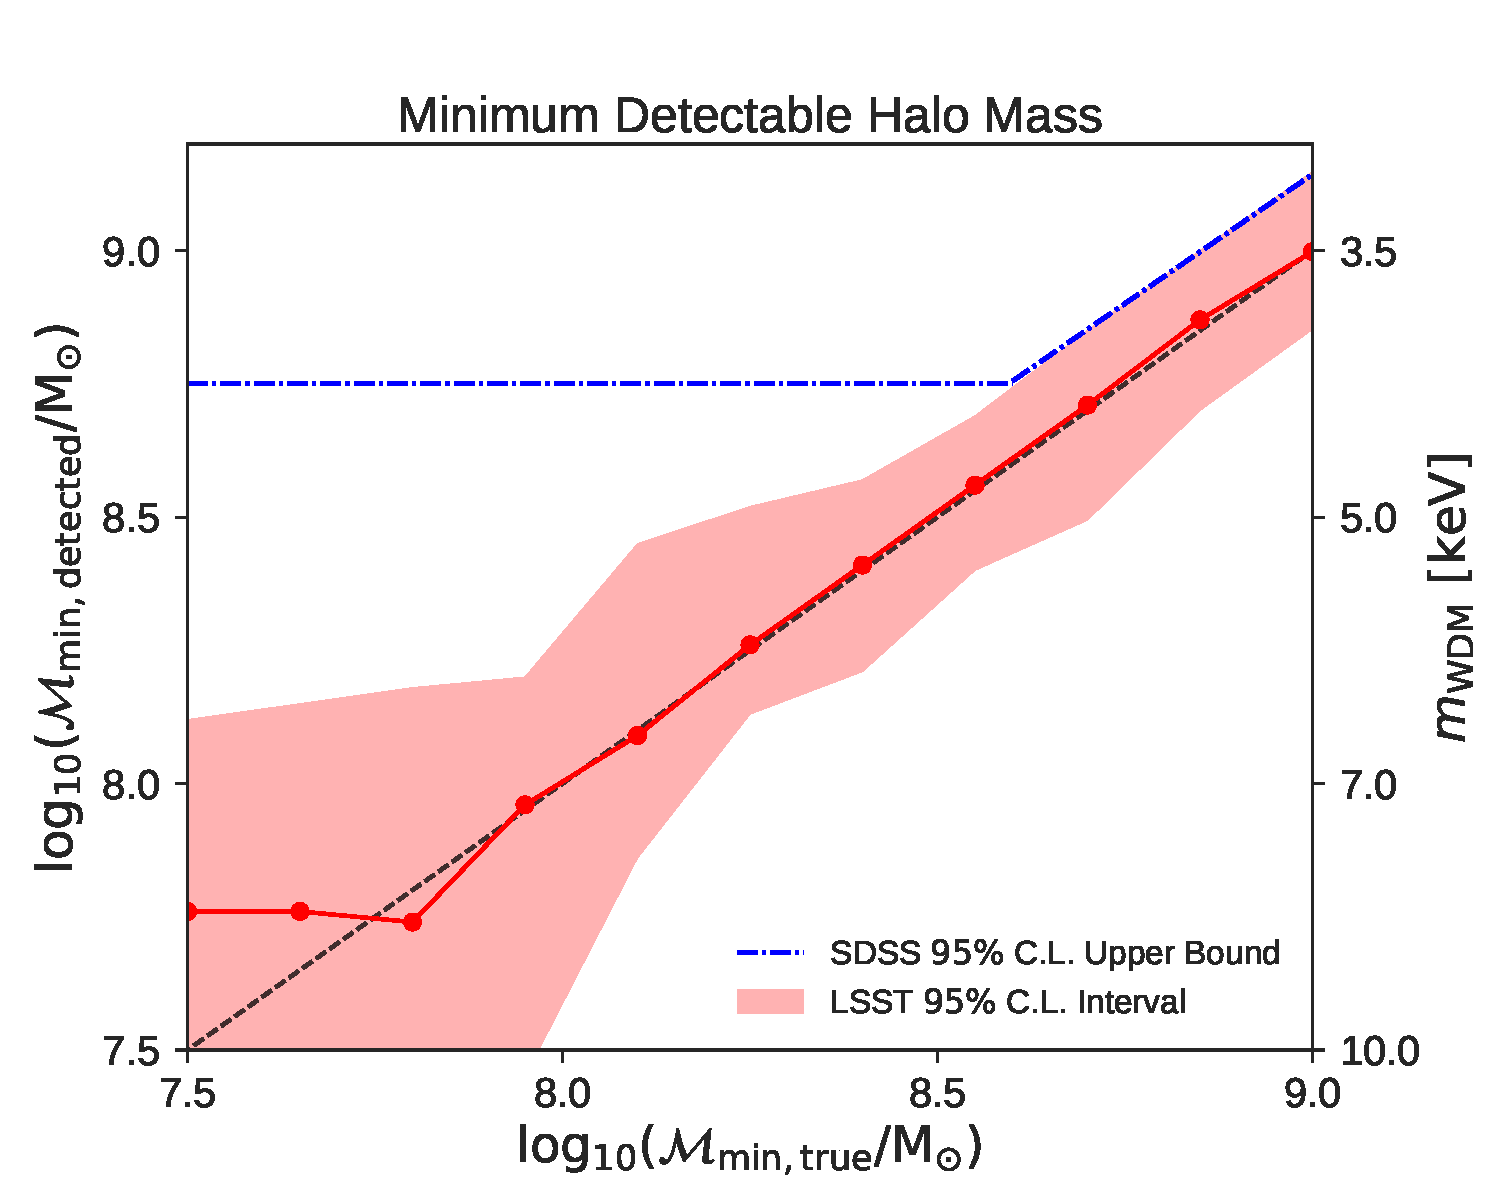
\includegraphics[width=0.49\textwidth]{figures/LSST_Mmin.pdf}
%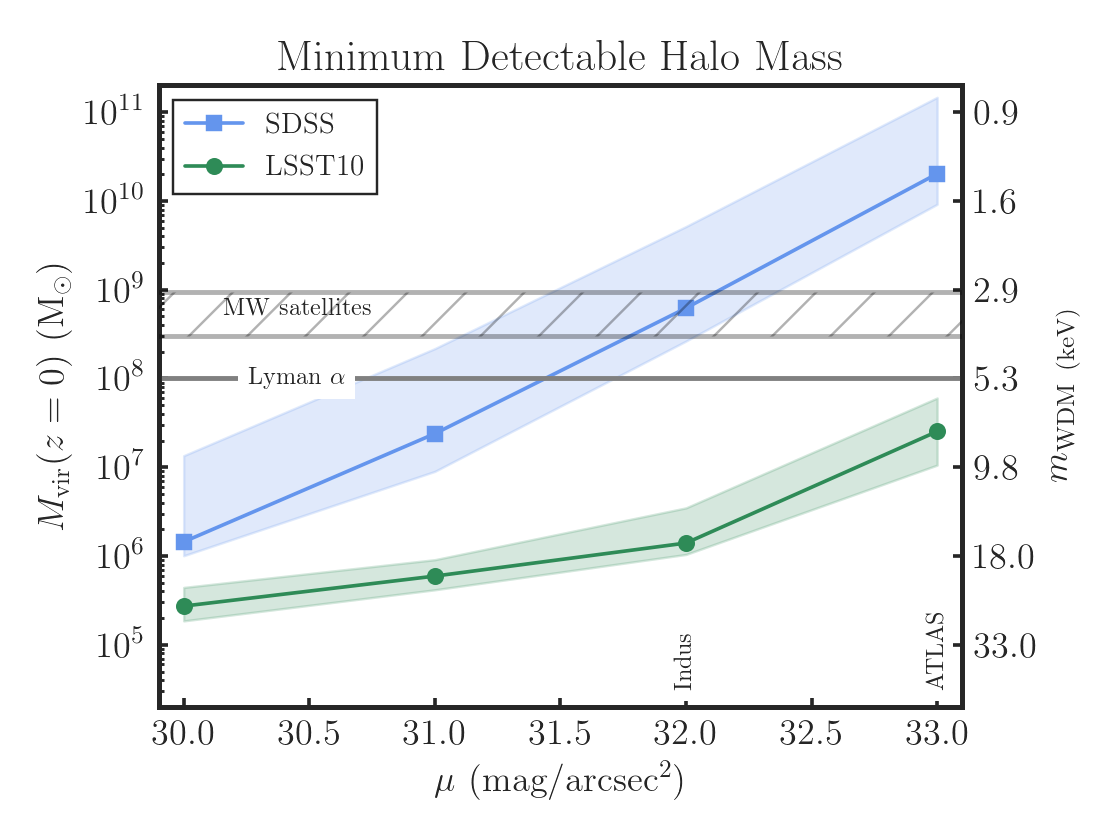
\includegraphics[width=0.49\textwidth]{figures/streamgap_constraints_3.png}
%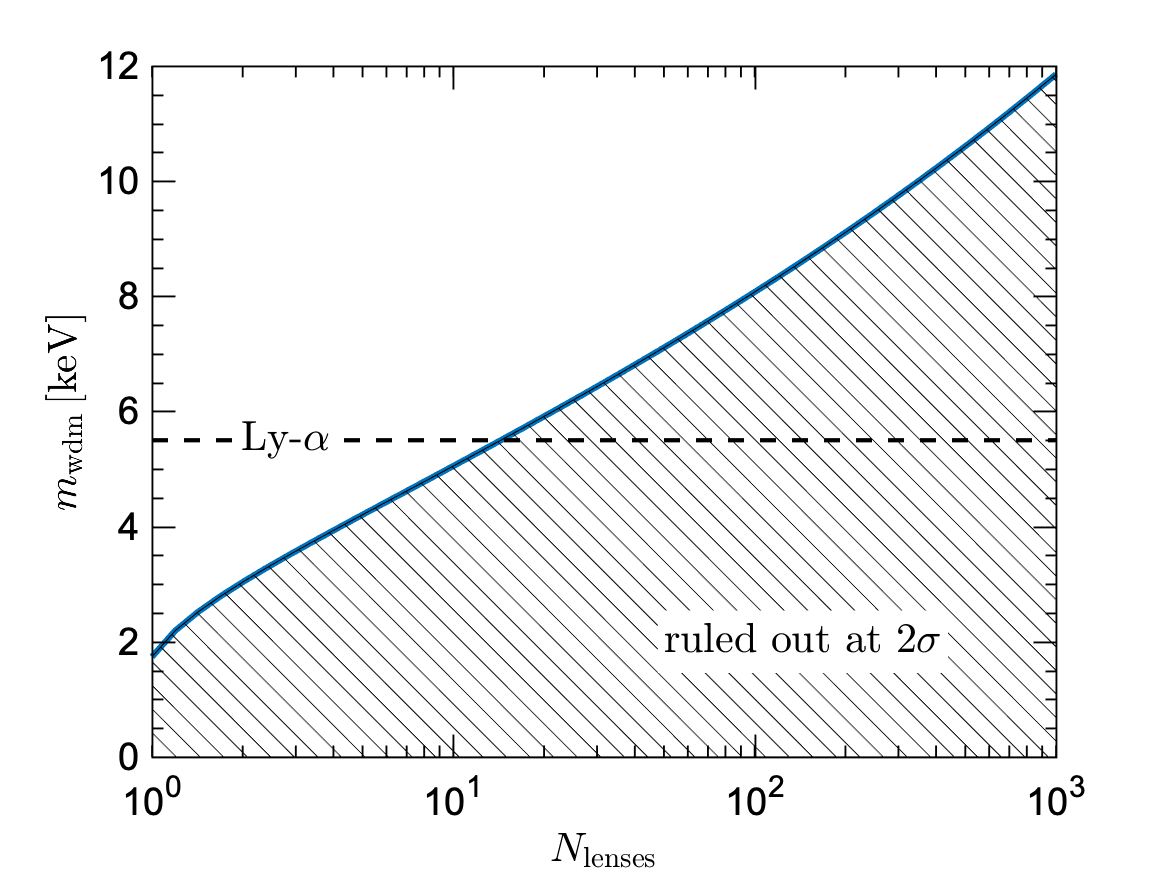
\includegraphics[width=0.50\textwidth]{figures/wdm_constraints_yh.png}
%\caption{Three complementary probes of minimum dark matter halo mass.}
%\end{figure}

%\begin{figure}
%    \centering
%    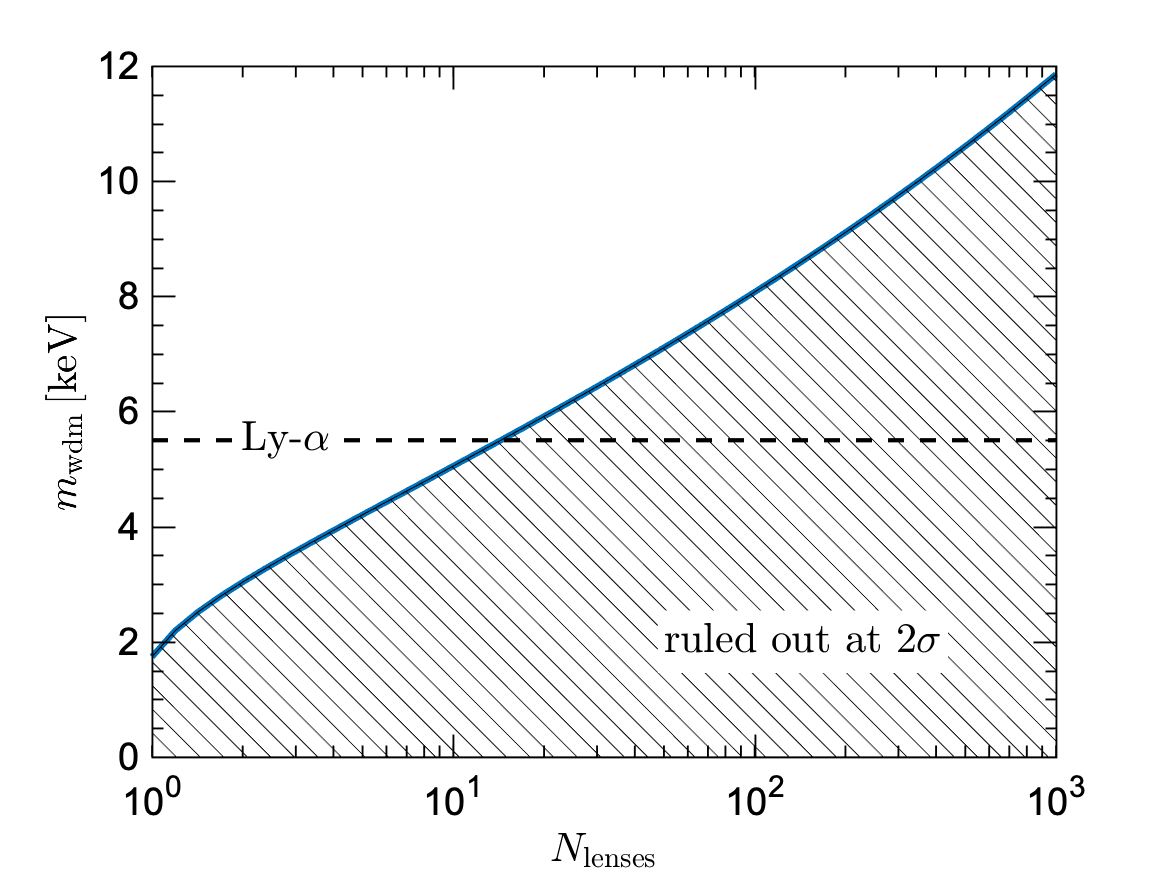
\includegraphics[width=0.50\textwidth]{figures/wdm_constraints_yh.png}
%    \caption{ \label{fig:lensing_wdmlim_vs_nlens} Projected $2\sigma$ constraints on WDM particle mass as a function of the number of strong lens systems that achieve a given (sub)halo mass detection threshold, under the assumption that CDM is correct. These constraints include only the contribution from halo substructure, and do not include the line-of-sight contribution.
%Exisiting Lyman-$\alpha$ forest constraints are shown with a dashed horizontal line \citep{2017PhRvD..96b3522I}. Figure based on \citet{Hezaveh_2016ltk}.
%}
%\end{figure}

%\begin{figure}[t]
%\centering
%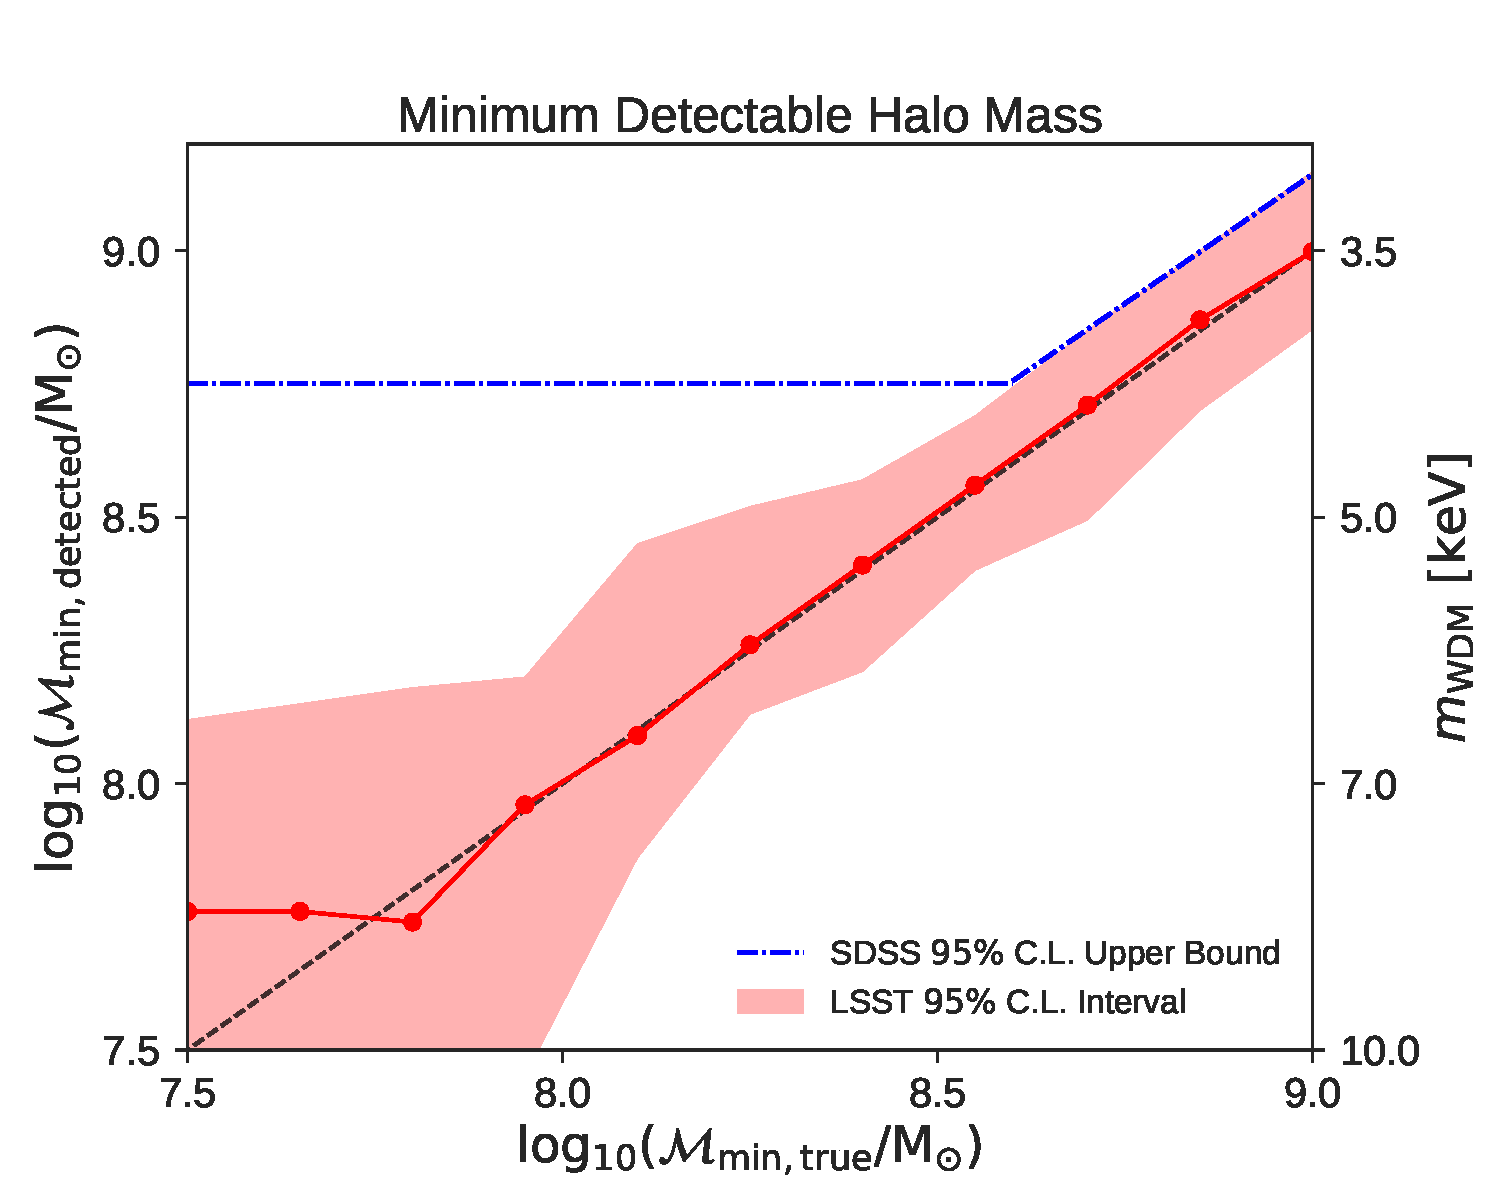
\includegraphics[width=0.775\textwidth]{figures/LSST_Mmin.pdf}
%\caption{Forecast for the minimum dark matter subhalo mass probed by LSST via observations of Milky Way satellites. The red band shows the $95\%$ confidence interval from our MCMC fits to mock satellite populations as a function of the true peak subhalo mass necessary for galaxy formation. Note that we marginalize over the relevant nuisance parameters associated with the galaxy--halo connection---including the effects of baryons using a model calibrated on subhalo disruption in hydrodynamic simulations \citep{2018ApJ...859..129N}---in our sampling. We indicate the corresponding constraints on the warm dark matter mass assuming $M_{\rm hm} = \mathcal{M}_{\rm{min}}$ (see \secref{wdm})}\label{fig:satellite_mmin}
%\end{figure}

%\begin{figure}[t]
%\centering
%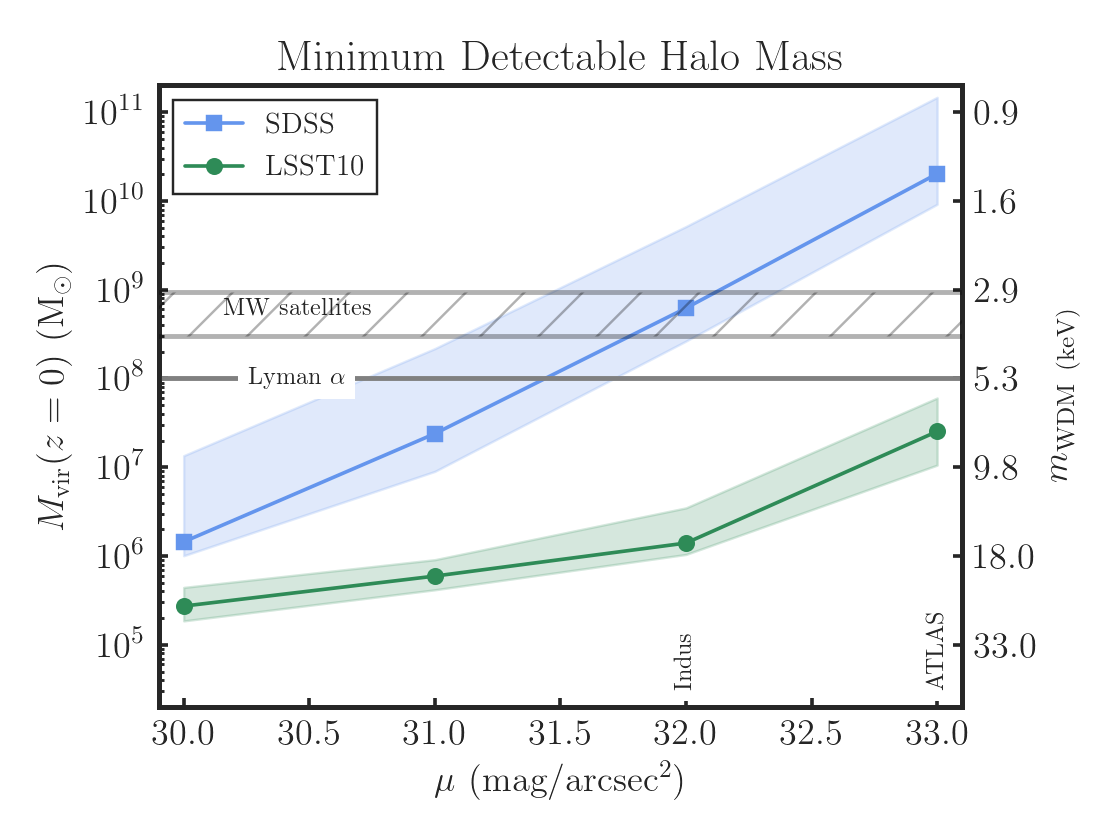
\includegraphics[width=0.85\textwidth]{figures/streamgap_constraints_3.png}
%\caption{\label{fig:streamsurveys} Detection limits for gaps formed from subhalos of different masses using photometry from SDSS (blue) or the 10-year LSST stack (green) as a function of the stream surface brightness.
%Shaded regions correspond to a 10-40 kpc distance range, with the lines representing 20 kpc. For streams with surface brightnesses similar to those found in DES, 32--$33 \magn \asec^{-2}$, LSST is expected to probe halo masses two to three orders of magnitude smaller than SDSS and substantially improve the current constraints from Milky Way satellites \citep{Nadler:2018, Jethwa:2018,Kim:2017iwr} and the Lyman-$\alpha$ forest \citep{2017PhRvD..96b3522I}. 
%We connect the detected halos to the mass of the warm dark matter particle that would produce a minimum halo of that mass using the relationship determined by \cite{Bullock:2017}. Note that the halo mass definition used here is the $z=0$ virial mass; to relate this quantity to the peak subhalo mass used in our warm dark matter constraints, we have assumed the best-case scenario of no tidal mass loss.
%}
%\end{figure}
\vspace{-1em} \subsection*{Périmètre IN2P3 et synergies} \vspace{-0.5em}

La collaboration scientifique DESC a pris récemment acte du fait que la caractérisation de la matière noire avec LSST recouvre très largement les problématiques scientifiques et techniques qui se posent dans le cadre de la caractérisation de l'énergie noire, son sujet central.
De la même manière, un programme de recherche soutenu de l'IN2P3 sur l'identification de la matière noire avec LSST est en parfaite adéquation avec son objectif principal de retour scientifique, qui porte également sur l'énergie noire. D'ailleurs deux des sondes discutées plus haut sont des sujets traités depuis longtemps au sein de l'institut.

\noindent {\bf Le microlensing} 
Cette voie de détection de matière noire sous forme d'objets compacts a été initiée aux USA et en France, notamment par l'IN2P3 au début des
années 1990 avec l'expérience EROS (Expérience de Recherche d'Objets Sombres).
Les relevés passés (EROS, MACHO) et actuels (MOA et OGLE) à la recherche d'effets de microlentille gravitationnelle ont exclu que la matière noire galactique soit majoritairement constituée d'objets compacts de masse inférieure à $10\Msun$ \citep{Tisserand2007,OGLE2010}. Or, les premières détections d'ondes gravitationnelles ont mis en évidence l'existence d'objets plus lourds que cette limite \citep{GW1,Bird}.
Le facteur limitant la sensibilité des relevés précédents à de tels objets est l'effondrement de
l'efficacité de détection des effets de lentille de longue durée (plusieurs années) qu'ils induisent.
Des travaux sont en cours actuellement à l'IN2P3 pour combiner les données des relevés passés, afin de bénéficier d'une plus grande couverture temporelle, et
de récupérer une efficacité raisonnable de détection des événements dus à d'éventuels trous noirs de masse intermédiaire \citep{MEMO}.
Ces travaux trouvent leur prolongement naturel dans la préparation de la stratégie d'échantillonnage et de
l'analyse des données temporelles de LSST en direction des champs stellaires (LMC, SMC et plan galactique), dans le cadre
des activités "transient" de LSST, en marge de DESC.
Comme l'efficacité de détection pour des événements de longue durée dépendra peu des détails de l'échantillonnage temporel, il faudra essentiellement
s'assurer que les intervalles entre mesures d'un même champ ne dépassent pas une saison. Nos études ont montré que,
après 10 années consécutives d'observation, on s'attend à ce que
les courbes de lumière mesurées dans LSST permettent d'estimer la contribution des objets de masse comprise entre
10 et $1000\Msun$ à la masse noire de la Voie Lactée \citep{MEMO}. Le savoir-faire maintenu à l'IN2P3 permettra en plus
de combiner les données de LSST avec celles des relevés historiques, ce qui fournira quelques millions de courbes de lumière
étalées sur plus de 40 années, et constituera un atout décisif pour les études d'efficacité, particulièrement délicates dans
la science du microlensing.

\noindent {\bf L'étude des galaxies naines sphéroïdes} Ces systèmes sont parmi les plus intéressants pour rechercher un signal indirect de présence de matière noire, en particulier dans la gamme des rayons gamma de haute et très haute énergie. En effet, ils sont proches, ont de grands rapports masse sur luminosité, et sont supposés être dénués de bruit de fond astrophysique en gamma (e.g. peu ou pas de gaz, ni de formation stellaire).
L'IN2P3 joue depuis longtemps un rôle important dans l'étude de ces objets avec le {\it Large Area Telescope} à bord de l'observatoire {\it Fermi} \citep[e.g.][]{1108.3546,1503.02641,2015MNRAS.453..849B,2017MNRAS.466..669C}, avec les instruments Tcherenkov H.E.S.S. et le futur observatoire CTA \citep[e.g.][]{Abramowski:2014tra,2019ICRC...36..539O,2019ICRC...36..542R}, ainsi que dans la phénoménologie de ces objets \citep[e.g.][]{2015MNRAS.446.3002B}. Les contraintes les plus récentes ont d'ailleurs été obtenus en partenariat avec la collaboration {\it Dark Energy Survey} (DES), qui a découvert plusieurs nouvelles galaxies naines dans le ciel sud. Avec LSST, plusieurs centaines de nouvelles naines avec une luminosité inférieure à $10^3\ L_\odot$ sont attendues \citep{Hargis:2014}, qui permettront à leur tour de mettre de nouvelles contraintes grâce aux données du LAT et de CTA.
Outre la découverte de nouvelles naines pour enrichir les catalogues de sources gamma potentielles, le simple comptage de ces sous-structures ainsi que l'étude de leur espace des phases fournit des contraintes directes sur la nature de la matière noire (voir plus haut).
Enfin, la détermination de leur profil de densité grâce à un suivi spectroscopique d'un sous-ensemble de galaxies naines sera également un outil discriminant important, par exemple entre SIDM et CDM \citep{2012MNRAS.423.3740V,Peter:2013,Nishikawa:2019lsc}.
L’enjeu des galaxies naines sphéroïdes et plus généralement des objets à faible luminosité de surface est donc de premier plan pour LSST, et l'IN2P3 a acquis une visibilité dans ce domaine, aussi bien observationnelle que théorique. 




Les deux exemples précédents montrent qu'une activité matière noire à l'IN2P3 au sein de LSST-France peut s'appuyer sur une expertise existante et une volonté affichée de participer au groupe de travail correspondant de DESC. Et cela, sans préjuger naturellement des intérêts que ne manqueront pas de susciter d'autres sondes observables par LSST, depuis les traînées stellaires, sur lesquelles le satellite Gaia fournit d'ores et déjà des données remarquables \citep{2018MNRAS.473.2060J,2018JCAP...07..061B}, jusqu'aux grandes structures, qui font l'objet de travaux français au sein de DESC \citep{2019arXiv190609042B,2019A&A...623A..76A,2017ApJ...845...28C}.

Ainsi, l'activité matière noire au sein de LSST-France entre naturellement dans la thématique ``astroparticules'', dont l'IN2P3 soutient fortement les efforts portant sur la détection directe, indirecte, ou sur collisionneur. D'ailleurs, LSST fournit une complémentarité importante avec de tels efforts. Les recherches indirectes d'un signal de matière noire avec des télescopes neutrino ou gamma \citep{Charles:2016,Albert:2017,1404.5503} pourront s'appuyer sur le gain en précision de la cartographie par LSST de la distribution de masse aux échelles galactiques et extra-galactiques. D'autres synergies entre ciel optique et ciel gamma sont d'ailleurs possibles, comme par exemple la recherche de corrélations entre relevé de galaxies et sources gamma \citep{2019arXiv190713484A}.
Pour ce qui est des efforts de détection directe, LSST étendra les mesures de cinématique locales obtenues par Gaia à de bien plus grandes distances, et sondera avec les observations de structures à petite échelle un régime de masse et de section efficace des candidats particules de matière noire inaccessibles aux mesures de détection directe \citep{drlica-wagner_2019_lsst_dark_matter}.
Notons également que LSST sera capable de suivre des événements extrêmes du ciel transitoire, parmi lesquels peut se cacher une signature de candidats matière noire comme les ALP ({\it axion-like particles}) \citep{2017PhRvL.118a1103M}. Or ces phénomènes extrêmes sont également un sujet traité à l'IN2P3\footnote{Nous mentionnons ici le livre blanc sur les synergies entre ondes gravitationnelles et matière noire \citep{2019arXiv190710610B}. Si le sujet n'est qu'indirectement lié à LSST, il souligne un peu plus à quel point l'IN2P3 par les projets qu'il soutient est au centre de la synergie à développer autour de la question transverse de l'identification de la matière noire.}.

Enfin, on ne saurait trop souligner l'importance d'encourager, en particulier au sein de l'IN2P3, les initiatives visant à réunir des communautés aux interfaces de l'astrophysique (dynamique galactique), de la cosmologie (formation des structures), et des astroparticules (modèles de matière noire et détections associées), comme l'atelier annuel ``News From The Dark Side'' du LUPM\footnote{Voir les sites des derniers ateliers pour plus d'informations: \href{https://indico.in2p3.fr/event/19035/}{2019}, \href{https://indico.in2p3.fr/event/17224/}{2018}, \href{https://indico.in2p3.fr/event/14497/}{https://indico.in2p3.fr/event/14497/}, et \href{https://indico.in2p3.fr/event/9143/}{2013}.}. 

\vspace{-1em} \subsection*{Conclusions} \vspace{-0.5em}

LSST commencera les opérations de science vers 2022. La France est très largement impliquée dans le projet, au niveau de la construction de la caméra et de la charge de calcul pour la réduction et l'analyse des données. Cette implication a historiquement trouvé son ancrage scientifique au sein de la communauté française intéressée par la question de l'énergie noire et membre de la {\it Dark Energy Science Collaboration} (DESC). DESC a récemment intégré un groupe de travail dédié à la matière noire, reconnaissant que cette thématique est indissolublement liée à celle de l'énergie noire\footnote{Le site de LSST considère le secteur sombre comme un seul axe thématique auquel LSST a été conçu pour répondre, voir \href{https://www.lsst.org/science}{https://www.lsst.org/science}. } et que les sondes ciblées et les outils d'analyse sont en grande partie semblables.
De son côté, l'IN2P3 a une riche contribution à la question essentielle de la nature de la matière noire (recherches directe, indirecte, sur collisionneur, et phénoménologie associée), et est idéalement positionné pour jouer un rôle important dans cette thématique avec LSST. Dans ce contexte, il est fortement souhaitable que l'IN2P3 soutienne l’association des axes de recherche sur l’énergie noire et sur la matière noire au sein de LSST-France, et joue un rôle prépondérant pour mieux structurer les différentes recherches associées. L'émergence de la communauté LSST matière noire à l'origine du livre blanc \citep{drlica-wagner_2019_lsst_dark_matter}, ainsi que l'initiative {\sc DarkMachine}\footnote{\href{https://darkmachines.org/}{https://darkmachines.org/}} sont autant d'exemples à l'étranger qui vont dans cette direction. 


%% In the 2020s, the impact of the LSST dark matter program will be enhanced by access to wide-field massively multiplexed spectroscopy on medium- to large-aperture telescopes ($\roughly 8$--$10$-meter class), deep spectroscopy on giant segmented mirror telescopes ($\roughly 30$-m class), together with high-resolution optical and radio imaging.
%% %with relatively smaller fields of view
%% Further theoretical work is also needed to interpret those observations in terms of particle models, to combine results from multiple observational methods, and to develop novel probes of dark matter.



\def\bibname{References}
\begingroup
  \small
  \setlength{\bibsep}{0pt plus 0.5ex}
  \bibliographystyle{JHEP}
  %\bibliographystyle{yahapj}
  \bibliography{main}
\endgroup

%\clearpage
%% \subsection*{Affiliations}
%% 
%%%%%%%%%%%%%%%%%%%%%%%%%%%%%%%%%%%%%%%%%%%%%%%%%%%%%%%%%%%%
%                                                          %
% Institutional aliases file.                              %
% Originally used in CV DM whitepaper,                     %
% successfully stolen for CV 21cm roadmap whitepaper,      %
% now to live a life of its own.                           %
%                                                          %
% When editing, please respect alphabetical ordering       %
% and avoid duplication (that is the entire point).        %
%                                                          %
%                                                          %
% A summer river being crossed                             %
% how pleasing                                             %
% with sandals in my hands!                                %
%       Yosa Buson (1716-1784)                             %
%                                                          %
%%%%%%%%%%%%%%%%%%%%%%%%%%%%%%%%%%%%%%%%%%%%%%%%%%%%%%%%%%%%

\newcommand{\Amherst}{University of Massachusetts, Amherst, MA 01003 USA}
\newcommand{\ANLHEP}{HEP Division, Argonne National Laboratory, Lemont, IL 60439, USA}
\newcommand{\APC}{Laboratoire Astroparticule et Cosmologie (APC), CNRS/IN2P3, Universit\'e Paris Diderot, 10, rue Alice Domon et Léonie Duquet, 75205 Paris Cedex 13, France}
\newcommand{\ASU}{Arizona State University, Tempe, AZ  85287}
\newcommand{\BenGurion}{Department of Physics, Ben-Gurion University, Be'er Sheva 84105, Israel}
\newcommand{\BNL}{Brookhaven National Laboratory, Upton, NY 11973}
\newcommand{\Brown}{Brown University, Providence, RI 02912}
\newcommand{\Bub}{Boston University, Boston, MA 02215}
\newcommand{\BU}{Boston University, Boston, MA 02215}
\newcommand{\Buffalo}{Department of Physics, University at Buffalo, SUNY Buffalo, NY 14260 USA}
\newcommand{\Caltech}{California Institute of Technology, Pasadena, CA 91125}
\newcommand{\Cardiff}{School of Physics and Astronomy, Cardiff University, The Parade, Cardiff, CF24 3AA, UK}
\newcommand{\Carleton}{Carleton University, K1S 5B6 Ottawa, Canada}
\newcommand{\Carnegie}{The Observatories of the Carnegie Institution for Science, 813 Santa Barbara St., Pasadena, CA 91101, USA}
\newcommand{\Cavendish}{Astrophysics Group, Cavendish Laboratory, J.J.Thomson Avenue, Cambridge, CB3 0HE, UK}
\newcommand{\CCA}{Center for Computational Astrophysics, 162 5th Ave, 10010, New York, NY, USA}
\newcommand{\CPPM}{Aix Marseille Univ, CNRS/IN2P3, CPPM, Marseille, France}
\newcommand{\CEADAP}{D\'epartement d’Astrophysique, CEA Saclay DSM/Irfu, 91191 Gif-sur-Yvette, France}
\newcommand{\CERN}{CERN, Geneva, Switzerland}
\newcommand{\CfA}{Harvard-Smithsonian Center for Astrophysics, MA 02138}
\newcommand{\CFT}{Center for Theoretical Physics, Polish Academy of Sciences, al. Lotnik\'{o}w 32/46, 02-668, Warsaw, Poland}
\newcommand{\Cincinnati}{University of Cincinnati, Cincinnati, OH 45221}
\newcommand{\CITA}{Canadian Institute for Theoretical Astrophysics, University of Toronto, Toronto, ON M5S 3H8, Canada}
\newcommand{\CNRSA}{CNRS, Laboratoire d'Annecy-le-Vieux de Physique Th\'{e}orique, France}
\newcommand{\CNYang}{C.N. Yang Institute for Theoretical Physics State University of New York Stony Brook, NY 11794}
\newcommand{\CMUCosmo}{Department 
of Physics, McWilliams Center for Cosmology, Carnegie Mellon University}
\newcommand{\Columbia}{Columbia University, New York, NY 10027}
\newcommand{\Cornell}{Cornell University, Ithaca, NY 14853}
\newcommand{\CPthree}{CP3-Origins, 5230 Odense, Denmark}
\newcommand{\CWRU}{Case Western Reserve University, Cleveland, OH 44106}
\newcommand{\daa}{Department of Astronomy and Astrophysics, University of Toronto, ON, M5S3H4}
\newcommand{\damtp}{DAMTP, Centre for Mathematical Sciences, Wilberforce Road, Cambridge, UK, CB3 0WA}
\newcommand{\DESY}{DESY,  22607 Hamburg, Germany}
\newcommand{\DFI}{Departamento de F\'isica, FCFM, Universidad de Chile, Blanco Encalada 2008, Santiago, Chile}
\newcommand{\DOE}{US. Department of Energy, Germantown, MD 20874}
\newcommand{\drexel}{Drexel University, Philadelphia, PA 19104}
\newcommand{\Duke}{Duke University and Triangle Universitites Nuclear Laboratory, Durham, NC 27708}
\newcommand{\DukePhys}{Department of Physics, Duke University, Durham, NC 27708, USA}
\newcommand{\dunlap}{Dunlap Institute for Astronomy and Astrophysics, University of Toronto, ON, M5S3H4}
\newcommand{\Durham}{Department of Physics, Lower Mountjoy, South Rd, Durham DH1 3LE, United Kingdom}
\newcommand{\ED}{University of Edinburgh, EH8 9YL Edinburgh, United Kingdom}
\newcommand{\EPFL}{Institute of Physics, Laboratory of Astrophysics, Ecole Polytechnique Fédérale de Lausanne (EPFL), Observatoire de Sauverny, 1290 Versoix, Switzerland}
\newcommand{\ETH}{ETH Zurich, Institute for Particle Physics, 8093 Zurich, Switzerland}
\newcommand{\FNAL}{Fermi National Accelerator Laboratory, Batavia, IL 60510}
\newcommand{\FQAUB}{Dept. de F\' isica Qu\` antica i Astrof\' isica, Universitat de Barcelona, Mart\' i i Franqu\` es 1, E08028 Barcelona, Spain}
\newcommand{\FSU}{Florida State University, Tallahassee, FL 32306}
\newcommand{\Glasgow}{University of Glasgow, G12 8QQ Glasgow, United Kingdom}
\newcommand{\GRAPPA}{GRAPPA Institute, University of Amsterdam, Science Park 904, 1098 XH Amsterdam, The Netherlands}
\newcommand{\GSFC}{Goddard Space Flight Center, Greenbelt, MD 20771 USA}
\newcommand{\GWU}{George Washington University, Washington, DC 20052}
\newcommand{\Hampton}{Hampton University, Hampton, VA 23668}
\newcommand{\HarvardPhys}{Department of Physics, Harvard University, Cambridge, MA 02138, USA}
\newcommand{\Haverford}{Haverford College, 370 Lancaster Ave, Haverford PA, 19041, USA}
\newcommand{\Hawaii}{University of Hawaii, Honolulu, HI 96822}
\newcommand{\HKUST}{The Hong Kong University of Science and Technology, Hong Kong SAR, China}
\newcommand{\houston}{University of Houston, Houston, TX 77204}
\newcommand{\IAP}{Institut d'Astrophysique de Paris (IAP), CNRS \& Sorbonne University, Paris, France}
\newcommand{\IAS}{Institute for Advanced Study, Princeton, NJ 08540}
\newcommand{\IBS}{Institute for Basic Science (IBS), Daejeon 34051, Korea}
\newcommand{\ICC}{ICC, University of Barcelona, IEEC-UB, Mart\' i i Franqu\` es, 1, E08028 Barcelona, Spain}
\newcommand{\ICCD}{Institute for Computational Cosmology, Department of Physics, Durham University, South Road, Durham, DH1 3LE, UK}
\newcommand{\ICE}{Institute of Space Sciences (ICE, CSIC), Campus UAB, Carrer de Can Magrans, s/n, 08193 Barcelona, Spain}
\newcommand{\ICRR}{Institute for Cosmic Ray Resaerch, The University of Tokyo, 456 Higashi-Mozumi, Kamioka, Hida, Gifu 506-1205, Japan}
\newcommand{\ICTP}{International Centre for Theoretical Physics, Strada Costiera, 11, I-34151 Trieste, Italy}
\newcommand{\IFAE}{Institut de Fisica d’Altes Energies, The Barcelona Institute of Science and Technology, Campus UAB, 08193 Bellaterra (Barcelona), Spain}
\newcommand{\IFPU}{IFPU - Institute for Fundamental Physics of the Universe, Via Beirut 2, 34014 Trieste, Italy}
\newcommand{\IFT}{Instituto de Fisica Teorica UAM/CSIC, Universidad Autonoma de Madrid, 28049 Madrid, Spain}
\newcommand{\IFUNAM}{IFUNAM - Instituto de F\'{i}sica, Universidad Nacional Aut\'onoma de M\'etico, 04510 CDMX, M\'exico}
\newcommand{\IHEP}{Institute of High Energy Physics, Austrian Academy of Sciences, 1050 Vienna, Austria}
\newcommand{\Imperial}{Theoretical Physics, Blackett Laboratory, Imperial College, London, SW7 2AZ, U.K.}
\newcommand{\Indiana}{Indiana University, Bloomington, IN 47405}
\newcommand{\INAFOATs}{INAF - Osservatorio Astronomico di Trieste, Via G.B. Tiepolo 11, 34143 Trieste, Italy}
\newcommand{\INAFOAS}{INAF - Osservatorio di Astrofisica e Scienza dello Spazio di Bologna, via Piero Gobetti 93/3, I-40129 Bologna, Italy}
\newcommand{\INFNCag}{Istituto Nazionale di Fisica Nucleare, Sezione di Cagliari,  09126 Cagliari, Italy}
\newcommand{\INFNCat}{Istituto Nazionale di Fisica Nucleare, Sezione di Catania, 95125 Catania, Italy}
\newcommand{\INFNG}{Istituto Nazionale di Fisica Nucleare, Sezione di Genova, 16146 Genova, Italy}
\newcommand{\INFN}{INFN – National Institute for Nuclear Physics, Via Valerio 2, I-34127 Trieste, Italy}
\newcommand{\INFNFE}{Istituto Nazionale di Fisica Nucleare, Sezione di Ferrara, 40122, Italy }
\newcommand{\INFNLNF}{Istituto Nazionale di Fisica Nucleare, Laboratori Nazionali di Frascati, 00044 Frascati, Italy}
\newcommand{\INFNLNS}{Istituto Nazionale di Fisica Nucleare, Laboratori Nazionali del Sud, 95125 Catania, Italy}
\newcommand{\INFNN}{Istituto Nazionale di Fisica Nucleare, Sezione di Napoli, 80125 Napoli, Italy }
\newcommand{\INFNRM}{Istituto Nazionale di Fisica Nucleare, Sezione di Roma, 00185 Roma, Italy}
\newcommand{\INFNT}{Istituto Nazionale di Fisica Nucleare, Sezione di Torino, 10125, Italy }
\newcommand{\ioa}{Institute of Astronomy, University of Cambridge,Cambridge CB3 0HA, UK}
\newcommand{\IPP}{Institute for Particle Physics, BC V8W 3P6 Victoria, Canada}
\newcommand{\IPMU}{Kavli Insitute for the Physics and Mathematics of the Universe (WPI), University of Tokyo, 277-8583 Kashiwa , Japan}
\newcommand{\IPNL}{Universit\'e de Lyon, F-69622, Lyon, France; Universit\'e de Lyon 1, Villeurbanne; CNRS/IN2P3, Institut de Physique Nucl\'eaire de Lyon}
\newcommand{\IRFU}{IRFU, CEA, Universit\'e Paris-Saclay, F-91191 Gif-sur-Yvette, France}
\newcommand{\ITFA}{Institute for Theoretical Physics, University of Amsterdam, Science Park 904, 1098 XH Amsterdam, The Netherlands}
\newcommand{\IUCAA}{The Inter-University Centre for Astronomy and Astrophysics, Pune, 411007, India}
\newcommand{\Jerusalem}{Hebrew University of Jerusalem, 91904 Jerusalem, Israel}
\newcommand{\JHU}{Johns Hopkins University, Baltimore, MD 21218}
\newcommand{\JLAB}{Thomas Jefferson National Laboratory, Newport News, VA 23606}
\newcommand{\JPL}{Jet Propulsion Laboratory, California Institute of Technology, Pasadena, CA, USA}
\newcommand{\KASSI}{Korea Astronomy and Space Science Institute, Daejeon 34055, Korea}
\newcommand{\kavli}{Kavli Institute for Cosmology, Cambridge, UK, CB3 0HA}
\newcommand{\KIAS}{School of Physics, Korea Institute for Advanced Study, 85 Hoegiro, Dongdaemun-gu, Seoul 130-722, Korea}
\newcommand{\KICP}{Kavli Institute for Cosmological Physics, Chicago, IL 60637}
\newcommand{\KIPAC}{Kavli Institute for Particle Astrophysics and Cosmology, Stanford 94305}
\newcommand{\KINGS}{King's College London, WC2R 2LS London, United Kingdom}
\newcommand{\Kobe}{Kobe University, 657-8501 Kobe, Japan}
\newcommand{\KPH}{Johannes Gutenberg University, 55128 Mainz, Germany}
\newcommand{\KPMU}{University of Tokyo, 277-8583  Kashiwa , Japan}
\newcommand{\KSU}{Kansas State University, Manhattan, KS 66506}
\newcommand{\Lafayette}{Lafayette College, Easton, PA 18042}
\newcommand{\LANL}{Los Alamos National Laboratory, Los Alamos, NM 87545}
\newcommand{\LBL}{Lawrence Berkeley National Laboratory, Berkeley, CA 94720}
\newcommand{\Leiden}{Lorentz Institute, Leiden University, Niels Bohrweg 2,Leiden, NL 2333 CA, The Netherlands}
\newcommand{\Liverpool}{University of Liverpool,  L69 7ZE Liverpool , United Kingdom}
\newcommand{\LLNL}{Lawrence Livermore National Laboratory, Livermore, CA, 94550}
\newcommand{\LPC}{Universit\'e Clermont Auvergne, CNRS/IN2P3, Laboratoire de Physique de Clermont, F-63000 Clermont-Ferrand, France}
\newcommand{\LPNHE}{Sorbonne Universit\'e, Universit\'e Paris Diderot, CNRS/IN2P3, Laboratoire de Physique Nucl\'eaire et de Hautes Energies, LPNHE, 4 Place Jussieu, F-75252 Paris, France}
\newcommand{\McGill}{McGill University, Montreal, QC H3A 2T8, Canada}
\newcommand{\Melbourne}{School of Physics, The University of Melbourne, Parkville, VIC 3010, Australia}
\newcommand{\Mines}{Colorado School of Mines, Golden, CO 80401}
\newcommand{\MIT}{Massachusetts Institute of Technology, Cambridge, MA 02139}
\newcommand{\MPE}{Max-Planck-Institut f\"{u}r extraterrestrische Physik (MPE), Giessenbachstrasse 1, D-85748 Garching bei M\"unchen, Germany}
\newcommand{\MPIA}{Max-Planck-Institut f\"{u}r Astrophysik, Karl-Schwarzschild-Str. 1, 85741 Garching, Germany}
\newcommand{\MPP}{Max-Planck-Institut f\"{u}r Physik (Werner-Heisenberg-Institut), F\"ohringer Ring 6, D-80805 M\"unchen, Germany}
\newcommand{\LUPM}{Laboratoire Univers et Particules de Montpellier, Univ. Montpellier and CNRS, 34090 Montpellier, France}
\newcommand{\NAOC}{National Astronomical Observatories, Chinese Academy of Sciences, PR China}
\newcommand{\NCBJ}{National Center for Nuclear Research, Ul.Pasteura 7,Warsaw, Poland}
\newcommand{\NCU}{National Central University, Taoyuan City 32001, Taiwan (R.O.C.)}
\newcommand{\NCSU}{Physics Department, North Carolina State Universitym, 2401 Stinson Dr, Raleigh, NC 27607}
\newcommand{\ND}{University of Notre Dame,vNotre Dame, IN 46556}
\newcommand{\NIU}{Northern Illinois University, DeKalb, Illinois 60115}
\newcommand{\NMSU}{New Mexico State University, Las Cruces, NM 88003}
\newcommand{\NOAO}{National Optical Astronomy Observatory, 950 N. Cherry Ave., Tucson, AZ 85719 USA}
\newcommand{\Northwestern}{Northwestern University, Evanston, IL 60201}
\newcommand{\Nottingham}{University of Nottingham, NG7 2RD Nottingham, United Kingdom}
\newcommand{\NWU}{Northwestern University, Evanston, IL 60208}
\newcommand{\NYU}{New York University, New York, NY 10003}
\newcommand{\OK}{ University of Oklahoma, Norman, OK 73019}
\newcommand{\ORNL}{Oak Ridge National Laboratory, Oak Ridge, TN 37831}
\newcommand{\OSU}{The Ohio State University, Columbus, OH 43212}
\newcommand{\OU}{Department of Physics and Astronomy, Ohio University, Clippinger Labs, Athens, OH 45701, USA}
\newcommand{\OskarKlein}{Oskar Klein Centre for Cosmoparticle Physics, Stockholm University, AlbaNova, Stockholm SE-106 91, Sweden}
\newcommand{\Oxford}{The University of Oxford, Oxford OX1 3RH, UK}
\newcommand{\Oxy}{Occidental College, Los Angeles, CA 90041}
\newcommand{\ParisSud}{Universit\'{e} Paris-Sud, LAL, UMR 8607, F-91898 Orsay Cedex, France \& CNRS/IN2P3, F-91405 Orsay, France}
\newcommand{\PI}{Perimeter Institute, Waterloo, Ontario N2L 2Y5, Canada}
\newcommand{\Pitt}{University of Pittsburgh and PITT PACC, Pittsburgh, PA 15260}
\newcommand{\PNNL}{Pacific Northwest National Laboratory ,Richland, WA 99352}
\newcommand{\PNPI}{Petersburg Nuclear Physics Institute, 188300 Gatchina, Russia}
\newcommand{\Port}{Institute of Cosmology \& Gravitation, University of Portsmouth, Dennis Sciama Building, Burnaby Road, Portsmouth PO1 3FX, UK}
\newcommand{\Princeton}{Princeton University, Princeton, NJ 08544}
\newcommand{\PSU}{The Pennsylvania State University, University Park, PA 16802}
\newcommand{\Purdue}{Purdue University, West Lafayette, IN 47907}
\newcommand{\PW}{Participation Worldscope, Sedona, Arizona and Hong Kong, SAR PRC}
\newcommand{\Queens}{Queen's University , K7L 3N6 Kingston, Canada}
\newcommand{\Queensland}{The University of Queensland, School of Mathematics and Physics, QLD 4072, Australia}
\newcommand{\QMUL}{Queen Mary University of London, Mile End Road, London E1 4NS, United Kingdom}
\newcommand{\RAL}{Radio Astronomy Laboratory, University of California Berkeley, Berkeley, CA 94720, USA}
\newcommand{\Rice}{Department of Physics \& Astronomy, Rice University, Houston, Texas 77005, USA}
\newcommand{\RIT}{Rochester Institute of Technology}
\newcommand{\RomaS}{Dipartimento di Fisica, Universit\`{a} La Sapienza, P. le A. Moro 2, Roma, Italy}
\newcommand{\RUG}{Kapteyn Astronomical Institute, University of Groningen, P.O. Box 800, 9700 AV Groningen, The Netherlands}
\newcommand{\Rutgers}{Department of Physics and Astronomy, Rutgers, the State University of New Jersey, 136 Frelinghuysen Road, Piscataway, NJ 08854, USA}
\newcommand{\Sanford}{Sanford Underground Research Facility, Lead, SD 57754}
\newcommand{\Sassari}{Universit\`a di Sassari, 07100 Sassari,  Italy}
\newcommand{\SCIPP}{University of California at Santa Cruz, Santa Cruz, CA 95064}
\newcommand{\Sejong}{Department of Physics and Astronomy, Sejong University, Seoul, 143-747, Korea}
\newcommand{\Sheffield}{University of Sheffield, S3 7RH Sheffield, United Kingdom}
\newcommand{\SHAO}{Shanghai Astronomical Observatory (SHAO), Nandan Road 80, Shanghai 200030, China}
\newcommand{\Siena}{Siena College, 515 Loudon Road, Loudonville, NY 12211, USA}
\newcommand{\SISSA}{SISSA - International School for Advanced Studies, Via Bonomea 265, 34136 Trieste, Italy}
\newcommand{\SimonFraser}{Department of Physics, Simon Fraser University, Burnaby, British Columbia, Canada V5A 1S6}
\newcommand{\SLAC}{SLAC National Accelerator Laboratory, Menlo Park, CA 94025}
\newcommand{\SMU}{Southern Methodist University, Dallas, TX 75275}
\newcommand{\SNOLAB}{SNOLAB, Lively, ON P3Y 1N2, Canada}
\newcommand{\SoCal}{University of Southern California, CA 90089 }
\newcommand{\Stanford}{Stanford University, Stanford, CA 94305}
\newcommand{\StonyBrook}{Stony Brook University, Stony Brook, NY 11794}
\newcommand{\STSCI}{Space Telescope Science Institute, Baltimore, MD 21218}
\newcommand{\SUNYA}{University at Albany SUNY, Albany, NY 12222}
\newcommand{\SussexAstronomy}{Astronomy Centre, School of Mathematical and Physical Sciences, University of Sussex, Brighton BN1 9QH, United Kingdom}
\newcommand{\Syracuse}{Syracuse University, Syracuse, NY 13244}
\newcommand{\Tamu}{Texas AandM University, College Station, TX 77843 }
\newcommand{\Techsource}{Techsource Incorporated, Los Alamos, NM 87544}
\newcommand{\TelAviv}{Tel-Aviv University,  69978 Tel-Aviv, Israel}
\newcommand{\Temple}{Temple University, Philadelphia, PA 19122}
\newcommand{\TIFR}{Tata Institute of Fundamental Research, Homi Bhabha Road, Mumbai 400005 India}
\newcommand{\Tsinghua}{Department of Physics and Tsinghua Center for Astrophysics, Tsinghua University, Beijing 100084, P R China}
\newcommand{\TUM}{Technical University of Munich,  80333 Munich, Germany}
\newcommand{\UA}{University of Alabama, Tuscaloosa, AL 35487}
\newcommand{\UAS}{Department of Astronomy/Steward Observatory, University of Arizona, Tucson, AZ  85721}
\newcommand{\UAM}{Universidad Aut\'onoma de Madrid, 28049, Madrid, Spain}
\newcommand{\UBC}{University of British Columbia, Vancouver, BC V6T 1Z1, Canada}
\newcommand{\UCB}{Department of Astronomy, University of California Berkeley, Berkeley, CA 94720, USA}
\newcommand{\UCBP}{Department of Physics, University of California Berkeley, Berkeley, CA 94720, USA}
\newcommand{\UCBSSL}{Space Sciences Laboratory, University of California Berkeley, Berkeley, CA 94720, USA}
\newcommand{\UCD}{University of California at Davis, Davis, CA 95616}
\newcommand{\UChicago}{University of Chicago, Chicago, IL 60637}
\newcommand{\UCI}{University of California, Irvine, CA 92697}
\newcommand{\UCLA}{University of California at Los Angeles, Los Angeles,  CA 90095}
\newcommand{\UCL}{University College London, WC1E 6BT London, United Kingdom}
\newcommand{\UCR}{University of California at Riverside, Riverside, CA 92521}
\newcommand{\UCSB}{University of California at Santa Barbara, Santa Barbara, CA 93106}
\newcommand{\UCSC}{University of California at Santa Cruz, Santa Cruz, CA 95064}
\newcommand{\UCSD}{University of California San Diego, La Jolla, CA 92093}
\newcommand{\UFL}{University of Florida, Gainesville, FL 32611}
\newcommand{\UFN}{Universit\`a Federico II di Napoli, 80125 Napoli, Italy}
\newcommand{\UGTO}{Divisi\'on de Ciencias e Ingenier\'ias, Universidad de Guanajuato, Le\'on 37150, M\'exico}
\newcommand{\UKY}{University of Kentucky, Lexington, KY 40506}
\newcommand{\UMD}{University of Maryland, College Park, MD 20742
\newcommand{\UMiami}{University of Miami, Coral Gables, FL 33124}}
\newcommand{\UMich}{University of Michigan, Ann Arbor, MI 48109}
\newcommand{\UMN}{University of Minnesota, Minneapolis, MN 55455}
\newcommand{\UnB}{Instituto de F\'{i}sica, Universidade de Bras\'{i}lia, 70919-970, Bras\'{i}lia, DF, Brazil}
\newcommand{\UNC}{University of North Carolina at Chapel Hill, Chapel Hill, NC 27599}
\newcommand{\UNH}{University of New Hampshire, Durham, NH 03824}
\newcommand{\UNIMI}{Dipartimento di Fisica ``Aldo Pontremoli'', Universit\`a{} degli Studi di Milano, via Celoria 16, 20133 Milano, Italy}
\newcommand{\UNIPD}{Dipartimento di Fisica e Astronomia ``G. Galilei'',Universit\`a degli Studi di Padova, via Marzolo 8, I-35131, Padova, Italy}
\newcommand{\UNM}{University of New Mexico, Albuquerque, NM 87131}
\newcommand{\UNV}{University of Nevada, Reno, NV 89557}
\newcommand{\UoM}{Jodrell Bank Center for Astrophysics, School of Physics and Astronomy, University of Manchester, Oxford Road, Manchester, M13 9PL, UK}
\newcommand{\UPenn}{Department of Physics and Astronomy, University of Pennsylvania, Philadelphia, Pennsylvania 19104, USA}
\newcommand{\UR}{Department of Physics and Astronomy, University of Rochester, 500 Joseph C. Wilson Boulevard, Rochester, NY 14627, USA}
\newcommand{\UrbanaC}{Department of Physics, University of Illinois at Urbana-Champaign, Urbana, Illinois 61801, USA}
\newcommand{\USC}{The University of South Carolina, Columbia, SC 29208}
\newcommand{\USD}{The University of South Dakota, Vermillion, SD 57069}
\newcommand{\UTD}{University of Texas at Dallas, Texas 75080}
\newcommand{\Utenn}{The University of Tennessee, Knoxville, TN 37996}
\newcommand{\Utah}{University of Utah, Department of Physics and Astronomy, 115 S 1400 E, Salt Lake City, UT 84112, USA}
\newcommand{\UVA}{University of Virginia, Charlottesville, VA 22903}
\newcommand{\Uvic}{University of Victoria, BC V8P 5C2 Victoria, Canada}
\newcommand{\UWaterloo}{Department of Physics and Astronomy, University of Waterloo, 200 University Ave W, Waterloo, ON N2L 3G1, Canada}
\newcommand{\UWMadison}{Department of Physics, University of Wisconsin - Madison, Madison, WI 53706}
\newcommand{\UW}{University of Washington, Seattle 98195}
\newcommand{\UWC}{Department of Physics \& Astronomy, University of the Western Cape, Cape Town 7535, South Africa}
\newcommand{\Vanderbilt}{Physics \& Astronomy Department, Vanderbilt University, PMB 401807, 2301 Vanderbilt Place, Nashville, TN 37235}
\newcommand{\VSI}{Van Swinderen Institute for Particle Physics and Gravity, University of Groningen, Nijenborgh 4, 9747~AG~Groningen, The~Netherlands}
\newcommand{\VT}{Virginia Tech, Blacksburg, VA 24061}
\newcommand{\VUU}{Virginia Union University, Richmond, Virginia, 23220}
\newcommand{\WCA}{Centre for Astrophysics, University of Waterloo, Waterloo, Ontario N2L 3G1, Canada}
\newcommand{\Weizmann}{Weizmann Institute of Science, 76100 Rehovot, Israel}
\newcommand{\Wellesley}{Wellesley College, Wellesley, MA 02481}
\newcommand{\wiscIce}{University of Wisconsin, Madison, WI 53706}
\newcommand{\WM}{College of William and Mary, Newport News, VA 23606}
\newcommand{\WUSL}{Washington University in St Louis, St. Louis, MO 63130}
\newcommand{\WVU}{CSEE, West Virginia University, Morgantown, WV 26505, USA}
\newcommand{\WVUGWAC}{Center for Gravitational Waves and Cosmology, West Virginia University, Morgantown, WV 26505, USA}
\newcommand{\Wyoming}{Department of Physics and Astronomy, University of Wyoming, Laramie, WY 82071, USA}
\newcommand{\Yale}{Department of Physics, Yale University, New Haven, CT 06520}
\newcommand{\YorkU}{Department of Physics and Astronomy, York University, Toronto, Ontario M3J 1P3, Canada}



\begin{multicols}{2}
\scriptsize
\parskip=4pt

\affil{$^{1}$ \UWMadison}
\affil{$^{2}$ \FNAL}
\affil{$^{3}$ \KICP}
\affil{$^{4}$ \UChicago}
\affil{$^{5}$ \UCI}
\affil{$^{6}$ \damtp}
\affil{$^{7}$ \KIPAC}
\affil{$^{8}$ \NYU}
\affil{$^{9}$ \Durham}
\affil{$^{10}$ \LLNL}
\affil{$^{11}$ \KASSI}
\affil{$^{12}$ \SISSA}
\affil{$^{13}$ \IFPU}
\affil{$^{14}$ \INFN}
\affil{$^{15}$ \SLAC}
\affil{$^{16}$ \GRAPPA}
\affil{$^{17}$ \Leiden}
\affil{$^{18}$ \JHU}
\affil{$^{19}$ \Port}
\affil{$^{20}$ \UCR}
\affil{$^{21}$ \UCLA}
\affil{$^{22}$ \OskarKlein}
\affil{$^{23}$ \INAFOATs}
\affil{$^{24}$ \EPFL}
\affil{$^{25}$ \CfA}
\affil{$^{26}$ \LBL}
\affil{$^{27}$ \daa}
\affil{$^{28}$ \UAS}
\affil{$^{29}$ \Rutgers}
\affil{$^{30}$ \Stanford}
\affil{$^{31}$ \PI}
\affil{$^{32}$ \CNRSA}
\affil{$^{33}$ NASA Goddard Space Flight Center}
\affil{$^{34}$ \UCBP}
\affil{$^{35}$ \OU}
\affil{$^{36}$ \LUPM}
\affil{$^{37}$ \MPE}
\affil{$^{38}$ \CMUCosmo}
\affil{$^{39}$ Institute for Theoretical Particle Physics and Cosmology, RWTH Aachen University, Germany}
\affil{$^{40}$ Univ. Grenoble Alpes, USMB, CNRS, LAPTh, F-74940 Annecy, France}
\affil{$^{41}$ \HarvardPhys}
\affil{$^{42}$ \UNM}
\affil{$^{43}$ \Queensland}
\affil{$^{44}$ \IFUNAM'}
\affil{$^{45}$ \UoM}
\affil{$^{46}$ \JPL}
\affil{$^{47}$ Laboratory for Astroparticle Physics, University of Nova Gorica}
\affil{$^{48}$ Department of Physics, University of Surrey, UK}
\affil{$^{49}$ \UCD}
\affil{$^{50}$ \Oxford}
\affil{$^{51}$ \CITA}
\affil{$^{52}$ \kavli}
\affil{$^{53}$ \IFT}
\affil{$^{54}$ \ANLHEP}
\affil{$^{55}$ Physical Science Department, Barry University}
\affil{$^{56}$ \UFL}
\affil{$^{57}$ \UR}
\affil{$^{58}$ \UGTO}
\affil{$^{59}$ \Haverford}
\affil{$^{60}$ \CCA}
\affil{$^{61}$ \OSU}
\affil{$^{62}$ \dunlap}
\affil{$^{63}$ \VT}
\affil{$^{64}$ \UPenn}
\affil{$^{65}$ Yonsei University, Seoul, South Korea}
\affil{$^{66}$ \UCSC}
\affil{$^{67}$ \TIFR}
\affil{$^{68}$ \ioa}
\affil{$^{69}$ \Brown}
\affil{$^{70}$ \BenGurion}
\affil{$^{71}$ \UCL}
\affil{$^{72}$ \UCB}
\affil{$^{73}$ \NOAO}
\affil{$^{74}$ \UNIPD}
\affil{$^{75}$ \UCSD}
\affil{$^{76}$ \Princeton}
\affil{$^{77}$ \CNYang}
\affil{$^{78}$ \Pitt}
\affil{$^{79}$ \VSI}
\affil{$^{80}$ \ICTP}
\affil{$^{81}$ Laboratoire de l'Accélérateur Linéaire, IN2P3-CNRS, France}
\affil{$^{82}$ \IUCAA}
\affil{$^{83}$ \Siena}
\affil{$^{84}$ \Wyoming}
\affil{$^{85}$ \Caltech}
\affil{$^{86}$ \Yale}
\affil{$^{87}$ \BNL}
\affil{$^{88}$ \Tamu}
\affil{$^{89}$ \ETH}
\affil{$^{90}$ Center for Cosmology and AstroParticle Physics, The Ohio State University}
\affil{$^{91}$ Department of Astronomy, The Ohio State University}
\affil{$^{92}$ \RomaS}
\affil{$^{93}$ \INFNRM}
\affil{$^{94}$ \UNH}
\affil{$^{95}$ \STSCI}
\affil{$^{96}$ Laborat\'orio Interinstitucional de e-Astronomia - LIneA, Rua Gal. Jos\'e Cristino 77, Rio de Janeiro, RJ - 20921-400, Brazil}
\affil{$^{97}$ \Sejong}
\affil{$^{98}$ \KSU}
\affil{$^{99}$ Departamento de F\'isica Te\'orica, M-15, Universidad Aut\'onoma de Madrid, E-28049 Madrid, Spain}
\affil{$^{100}$ \StonyBrook}
\affil{$^{101}$ \SHAO}
\affil{$^{102}$ \Carnegie}
\affil{$^{103}$ \UMich}
\affil{$^{104}$ \MIT}
\affil{$^{105}$ INAF-Italian National Institute of Astrophysics, Italy}
\affil{$^{106}$ Space Telescope Science Institute}
\affil{$^{107}$ \DukePhys}
\affil{$^{108}$ \Duke}
\affil{$^{109}$ \UGTO'}
\affil{$^{110}$ \houston}
\affil{$^{111}$ \Syracuse}
\affil{$^{112}$ \MPIA}
\affil{$^{113}$ Center for Astrophysics and Cosmology, University of Nova Gorica}
\affil{$^{114}$ \ED}

\normalsize
\end{multicols}
\parskip=8pt




\end{document}

